%\documentclass[a4paper,10pt]{article}
\documentclass{llncs}
\usepackage[spanish]{babel}
\usepackage[utf8]{inputenc} %Si no lo agrego no se ven las letras con tilde
\usepackage{color,hyperref} % Para el mailto
\usepackage{listings} % Para agregar código de programación
\usepackage{graphicx}
\graphicspath{ {images/} }
\usepackage{float} % para usar [H]
\usepackage{multirow, array} % para las tablas
%\usepackage[tablename=Figura]{caption} % Si quiero cambiar el nombre de ``Cuadro'' que viene por defecto en las tablas

\hyphenation{he-rra-mien-ta es-cri-ban va-lor va-lo-res in-he-ren-te e-xis-ta} %Indico como deben dividirse las palabras que s e ``cortan'' mal cuando se justifica el texto
\newcommand{\mailPersonal}{j\_godoy@openmailbox.com}

%opening
\title{Generador de casos de Test automáticos a través de ejecución simbólica dinámica}
\author{Javier Ignacio Godoy \\ \href{mailto:\mailPersonal}{\mailPersonal} }
\institute{Instituto de Industria, Universidad Nacional de General Sarmiento, Buenos Aires, Argentina}


\begin{document}

\maketitle

%%%%%%%%%%%%%%%%%%%%%%%%%%%%%%%%%%%%%%%%%%%%%%%%%%%%%%%%%%%%%%%%%%%%%%%%
%				ABSTRACT			       %
%%%%%%%%%%%%%%%%%%%%%%%%%%%%%%%%%%%%%%%%%%%%%%%%%%%%%%%%%%%%%%%%%%%%%%%%
\begin{abstract}
Los casos de test unitarios son útiles para probar si la implementación de una función tiene el comportamiento esperado.
Si bien no se puede garantizar al 100\% la correcta implementación, los test nos dan mayor seguridad de su comportamiento,
además de permitir que futuras modificaciones en la implementación mantengan el comportamiento esperado al momento de hacer los test.
Sin embargo, la tarea de hacer los test manualmente es compleja y costosa, lo que lleva a muchos programadores a obviar esta tarea,
lo cual no es nada recomendable. La herramienta presentada en este artículo permite generar automáticamente casos de test unitarios
en el lenguaje Java garantizando cubrir todas las sentencias y todas las ramas (alcanzables) del programa.
\keywords{ejecución simbólica, test unitarios, ejecución concólica. test automáticos}
\end{abstract}



%%%%%%%%%%%%%%%%%%%%%%%%%%%%%%%%%%%%%%%%%%%%%%%%%%%%%%%%%%%%%%%%%%%%%%%%
%				INTRODUCCIÓN			       %
%%%%%%%%%%%%%%%%%%%%%%%%%%%%%%%%%%%%%%%%%%%%%%%%%%%%%%%%%%%%%%%%%%%%%%%%
\section{Introducción}
El desarrollo de software por lo general es complejo y su mantenimiento costoso. Es común que, al agregar o cambiar una funcionalidad, estemos generando un bug sin percatarnos de ello.
Esto puede provocar incluso la imposibilidad de mantener un producto de software, especialmente si los encargados de hacerlo no son quienes escribieron el código original.
Modificar implementaciones de terceros (o las propias luego de un tiempo de haberlas desarrollado) generalmente provoca temor de generar bugs o dejar inconsistente el sistema. 

JUnit, un framework Java para la ejecución de test unitarios, suele usarse para obtener ciertas garantías de que un programa Java se comporta de la forma esperada,
minimizando las consecuencias anteriormente mencionadas y mejorando la calidad del código. Lo recomendable es crear al menos un test por cada método implementado.
Mientras más test unitarios para cada método se escriban, mayor seguridad de su comportamiento se tendrá.
Implementar casos de test se considera esencial en las compañías de software para dar un producto de calidad a los clientes. Sin embargo, muchos programadores continúan escribiendo
código sin sus respectivos casos de test. Esto podría deberse por desconocimiento o debido al tiempo extra que requiere escribir los casos de test, aunque las ventajas que otorga
lo hacen necesario. Estudios sugieren que aproximadamente el 50\% del esfuerzo de desarrollar software está representado por el testing \cite{econImpact}, como una muestra de la
importancia y el esfuerzo que requiere esta disciplina.

Existen varios enfoques para tratar la generación de casos de test automáticos. Uno de estos es la generación de inputs aleatorios a partir de los cuales se crean los casos de test.
Entre sus ventajas se destacan la rapidez de generación de los test con una buena cobertura de código. Sin embargo, presenta al menos dos problemas importantes.
Por un lado, genera conjuntos de test cuyos inputs son redundantes \cite{cute}. Por otro lado, la probabilidad de seleccionar aleatoriamente un input particular que detecte un bug
en el código puede ser muy pequeña \cite{cute}. Por ejemplo, la rama verdadera del condicional “if ($x==10$) then ...” sólo tiene una chance de ser ejecutada sobre \(2^{32}\) si $x$
es un input del programa de tipo entero de 32 bit que es inicializado aleatoriamente \cite{dart}.
Otro de los enfoques utilizados es la ejecución simbólica: en lugar de ejecutar un programa usando valores concretos como inputs del mismo -números, por ejemplo-, se ejecuta con
representaciones simbólicas para un conjunto de clases de inputs \cite{symb}. Una ejecución simbólica está representado por valores simbólicos para los parámetros de entrada y una
fórmula -restricción- simbólica para el output. Cada expresión condicional en el programa representa una restricción que determina un camino en el árbol de ejecución.
Nótese que cada camino, en caso de tener solución factible, determina diferentes valores como inputs. Para analizar los diferentes caminos en el árbol de ejecución, se suele utilizar
backtracking. Sin embargo, para ejecuciones grandes y complejas, se vuelve computacionalmente difícil de llevar a cabo.

Un método similar a la ejecución simbólica para tratar la generaciónde test automáticos es el conocido como ejecución concólica. Como su palabra lo indica, es una técnica que une la
ejecución concreta con la simbólica; para cada valor concreto ingresado como input del programa (parámetros de una función), se registran los valores simbólicos de estos parámetros y
se mantiene el valor simbólico a través de las diferentes asignaciones que se realicen en el cuerpo del programa. Al igual que en la ejecución simbólica, cada camino del árbol de
ejecución determina una fórmula de las variables simbólicas representadas como restricciones para ese camino particular. En vez de utilizar backtracking,
las condiciones simbólicas de un determinado camino son utilizadas en un SMT Solver para obtener nuevos valores concretos que permitan recorrer un camino alternativo del programa.
Utilizando estos valores concretos como nuevos inputs del programa, y siguiendo una operación similar con el resto de los caminos del árbol de ejecución, se puede obtener un conjunto
de clases de inputs que funcionen como casos de test. El presente artículo describe una herramienta que utiliza esta técnica.


%%%%%%%%%%%%%%%%%%%%%%%%%%%%%%%%%%%%%%%%%%%%%%%%%%%%%%%%%%%%%%%%%%%%%%%%
%				Ejemplo			       	       %
%%%%%%%%%%%%%%%%%%%%%%%%%%%%%%%%%%%%%%%%%%%%%%%%%%%%%%%%%%%%%%%%%%%%%%%%
\section{Ejemplo}
A continuación se describe un ejemplo de cómo la herramienta construye los test para el método Java de la figura \ref{arbolEjecucion}.

Antes de comenzar la ejecución, el código es instrumentado de forma tal de ir manteniendo un mapeo entre las variables y sus valores simbólicos. Al iniciar la ejecución sobre el
código ya instrumentado, la herramienta asigna el valor cero a ambas variables. De esta forma, se tiene que $x=0, y=0$ como valores concretos y \(\{x\mapsto x_0,y\mapsto y_0\}\)
son las expresiones simbólicas asociadas. En la primer sentencia del método, se actualiza el valor de la variable x, por lo tanto, se actualizan las expresiones simbólicas
\(\{x\mapsto x_0+3,y\mapsto y_0\}\). Luego, la evaluación de la guarda del primer if da verdadero, y la del segundo da falso, y la ejecución de la función termina.
La herramienta recolecta las restricciones de los predicados condicionales ejecutados: $x_0+3 \geq y_0$ (del primer If) y $x_0+3 \leq 10$ (del segundo If).
Estas restricciones ($x_0+3 \geq y_0, x_0+3 \leq 10$) las llamaremos restricciones simbólicas. Luego se niega el último predicado ($x_0+3 > 10$) y se resuelven las restricciones
simbólicas para obtener un camino alternativo al ya recorrido. Estas restricciones se resuelven por medio de un SMT Solver: se envían las restricciones y devuelve valores
concretos para las variables simbólicas de forma tal que se satisfagan las ecuaciones. Para las restricciones $x_0+3 \geq y_0, x_0+3 > 10$ se proponen los valores $x_0 = 8, y_0 = 11$.

Se ejecuta otra vez el método toTest con estos valores, dando verdadero tanto el primer if como el segundo; por lo tanto ambas ramas ya han sido cubiertas y se descarta la condición
simbólica correspondiente a esa bifurcación, quedando todavía pendiente obtener valores que hagan falsa $x_0+3 \geq y_0$. Por lo tanto se niega esta condición obtenidendo
$x_0+3 < y_0$ y se le pide al Solver valores que la satisfaga. Este devuelve $x=-1, y=3$. Al ejecutar con estos valores el método, no se pasa el primer If, con lo que se termina de recorrer todos los posibles caminos del árbol de ejecución.

Finalmente, con los pares de valores \{($x=0,y=0$), ($x=8,y=11$), ($x=-1,y=3$)\} se crean tres test, uno por cada par de valores devuelto. En la figura 1 se muestra el árbol
de ejecución del método toTest. Cabe destacar que cada hoja del árbol representará un conjunto diferente de valores que funcionarán como input para testear dicho método,
asegurando el 100\% de cobertura de código alcanzable \footnote{Puede suceder que el método a testear contenga “código muerto”, es decir, código que jamás se ejecutará
independientemente de los valores de entrada de dicho método}, tanto de sentencias como de ramas. 


\begin{figure*}[hbt!]
  \centering
    \begin{minipage}[b]{0.5\textwidth}
      \begin{lstlisting}[language=Java]
	Integer toTest(int x, int y)
	{
	  x = x +3;
	    if(x>=y) 
	      if( x > 10) 
		return x;
	  return y;
	}
      \end{lstlisting}
      \centering{(a)}
    \end{minipage}
  \begin{minipage}[b]{0.45\textwidth}
    \centering
    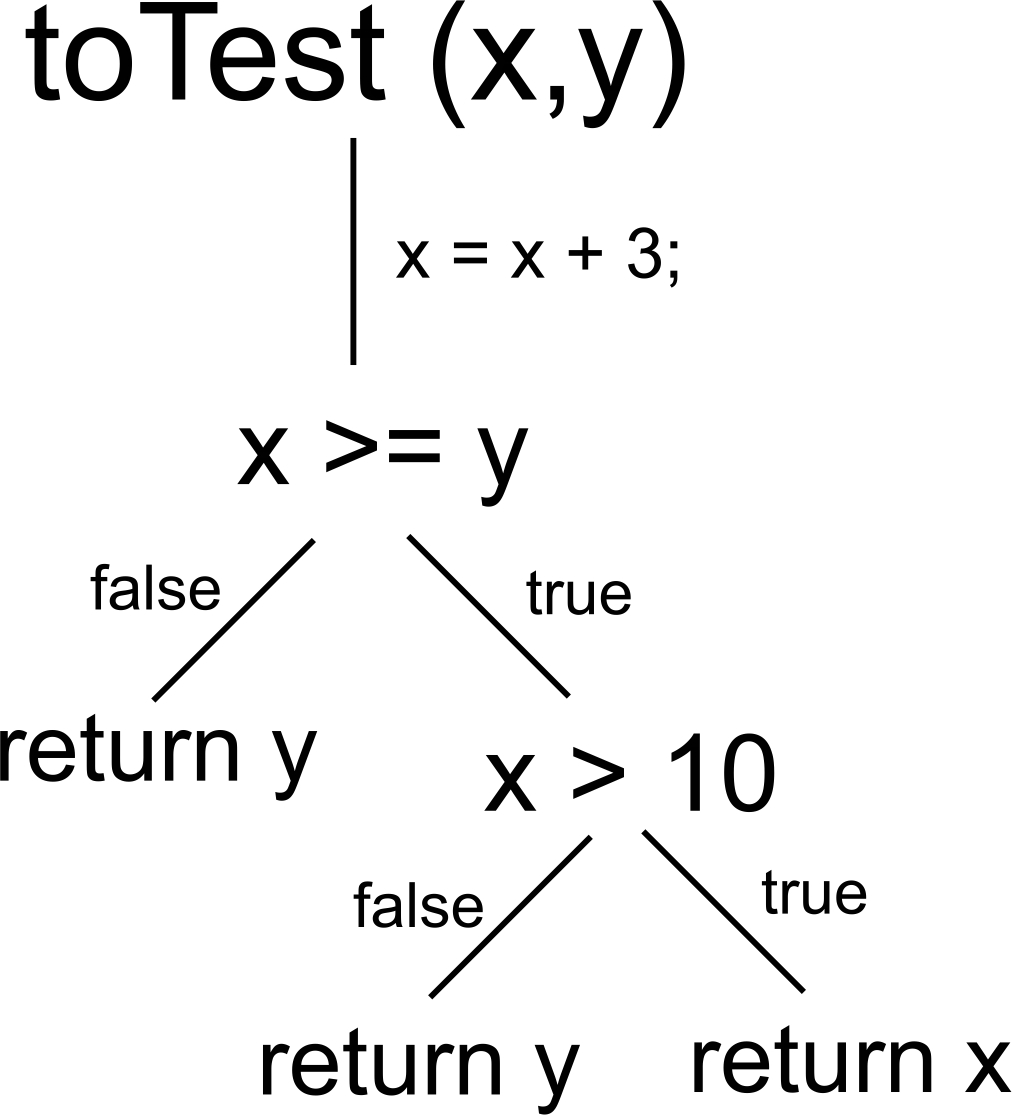
\includegraphics[width=0.6\textwidth]{arbolEjecucion}\\
    \centering{(b)}
  \end{minipage}
  \caption{Ejemplo de código Java (a) junto a su árbol de ejecución (b) correspondiente}
  \label{arbolEjecucion}
\end{figure*}


%%%%%%%%%%%%%%%%%%%%%%%%%%%%%%%%%%%%%%%%%%%%%%%%%%%%%%%%%%%%%%%%%%%%%%%%
%				El problema de los ciclos	       %
%%%%%%%%%%%%%%%%%%%%%%%%%%%%%%%%%%%%%%%%%%%%%%%%%%%%%%%%%%%%%%%%%%%%%%%%
\section{El problema de los ciclos}\label{sec:loopProblem}
Es importante destacar que el enfoque propuesto presenta un problema inherente a la ejecución simbólica al tratar con código que posea ciclos.
Este problema es que al iterar sobre una variable simbólica en un ciclo puede suceder que el mismo continúe indefinidamente al generar una nueva
ejecución en cada e\-va\-lua\-ción de la condición del ciclo. En la figura \ref{cicloInf} se muestra un ejemplo donde sucede esto:


\begin{figure*}[hbt!]
   \centering
    \begin{minipage}[H]{0.5\textwidth}
      \begin{lstlisting}[language=Java]
	Integer toTest2(int x)
	  {
	    int y = 0;
	    while (y < x)
	      y++;
	    return y;
	  }
      \end{lstlisting}
    \end{minipage}
  \begin{minipage}[H]{0.45\textwidth}
    \centering
    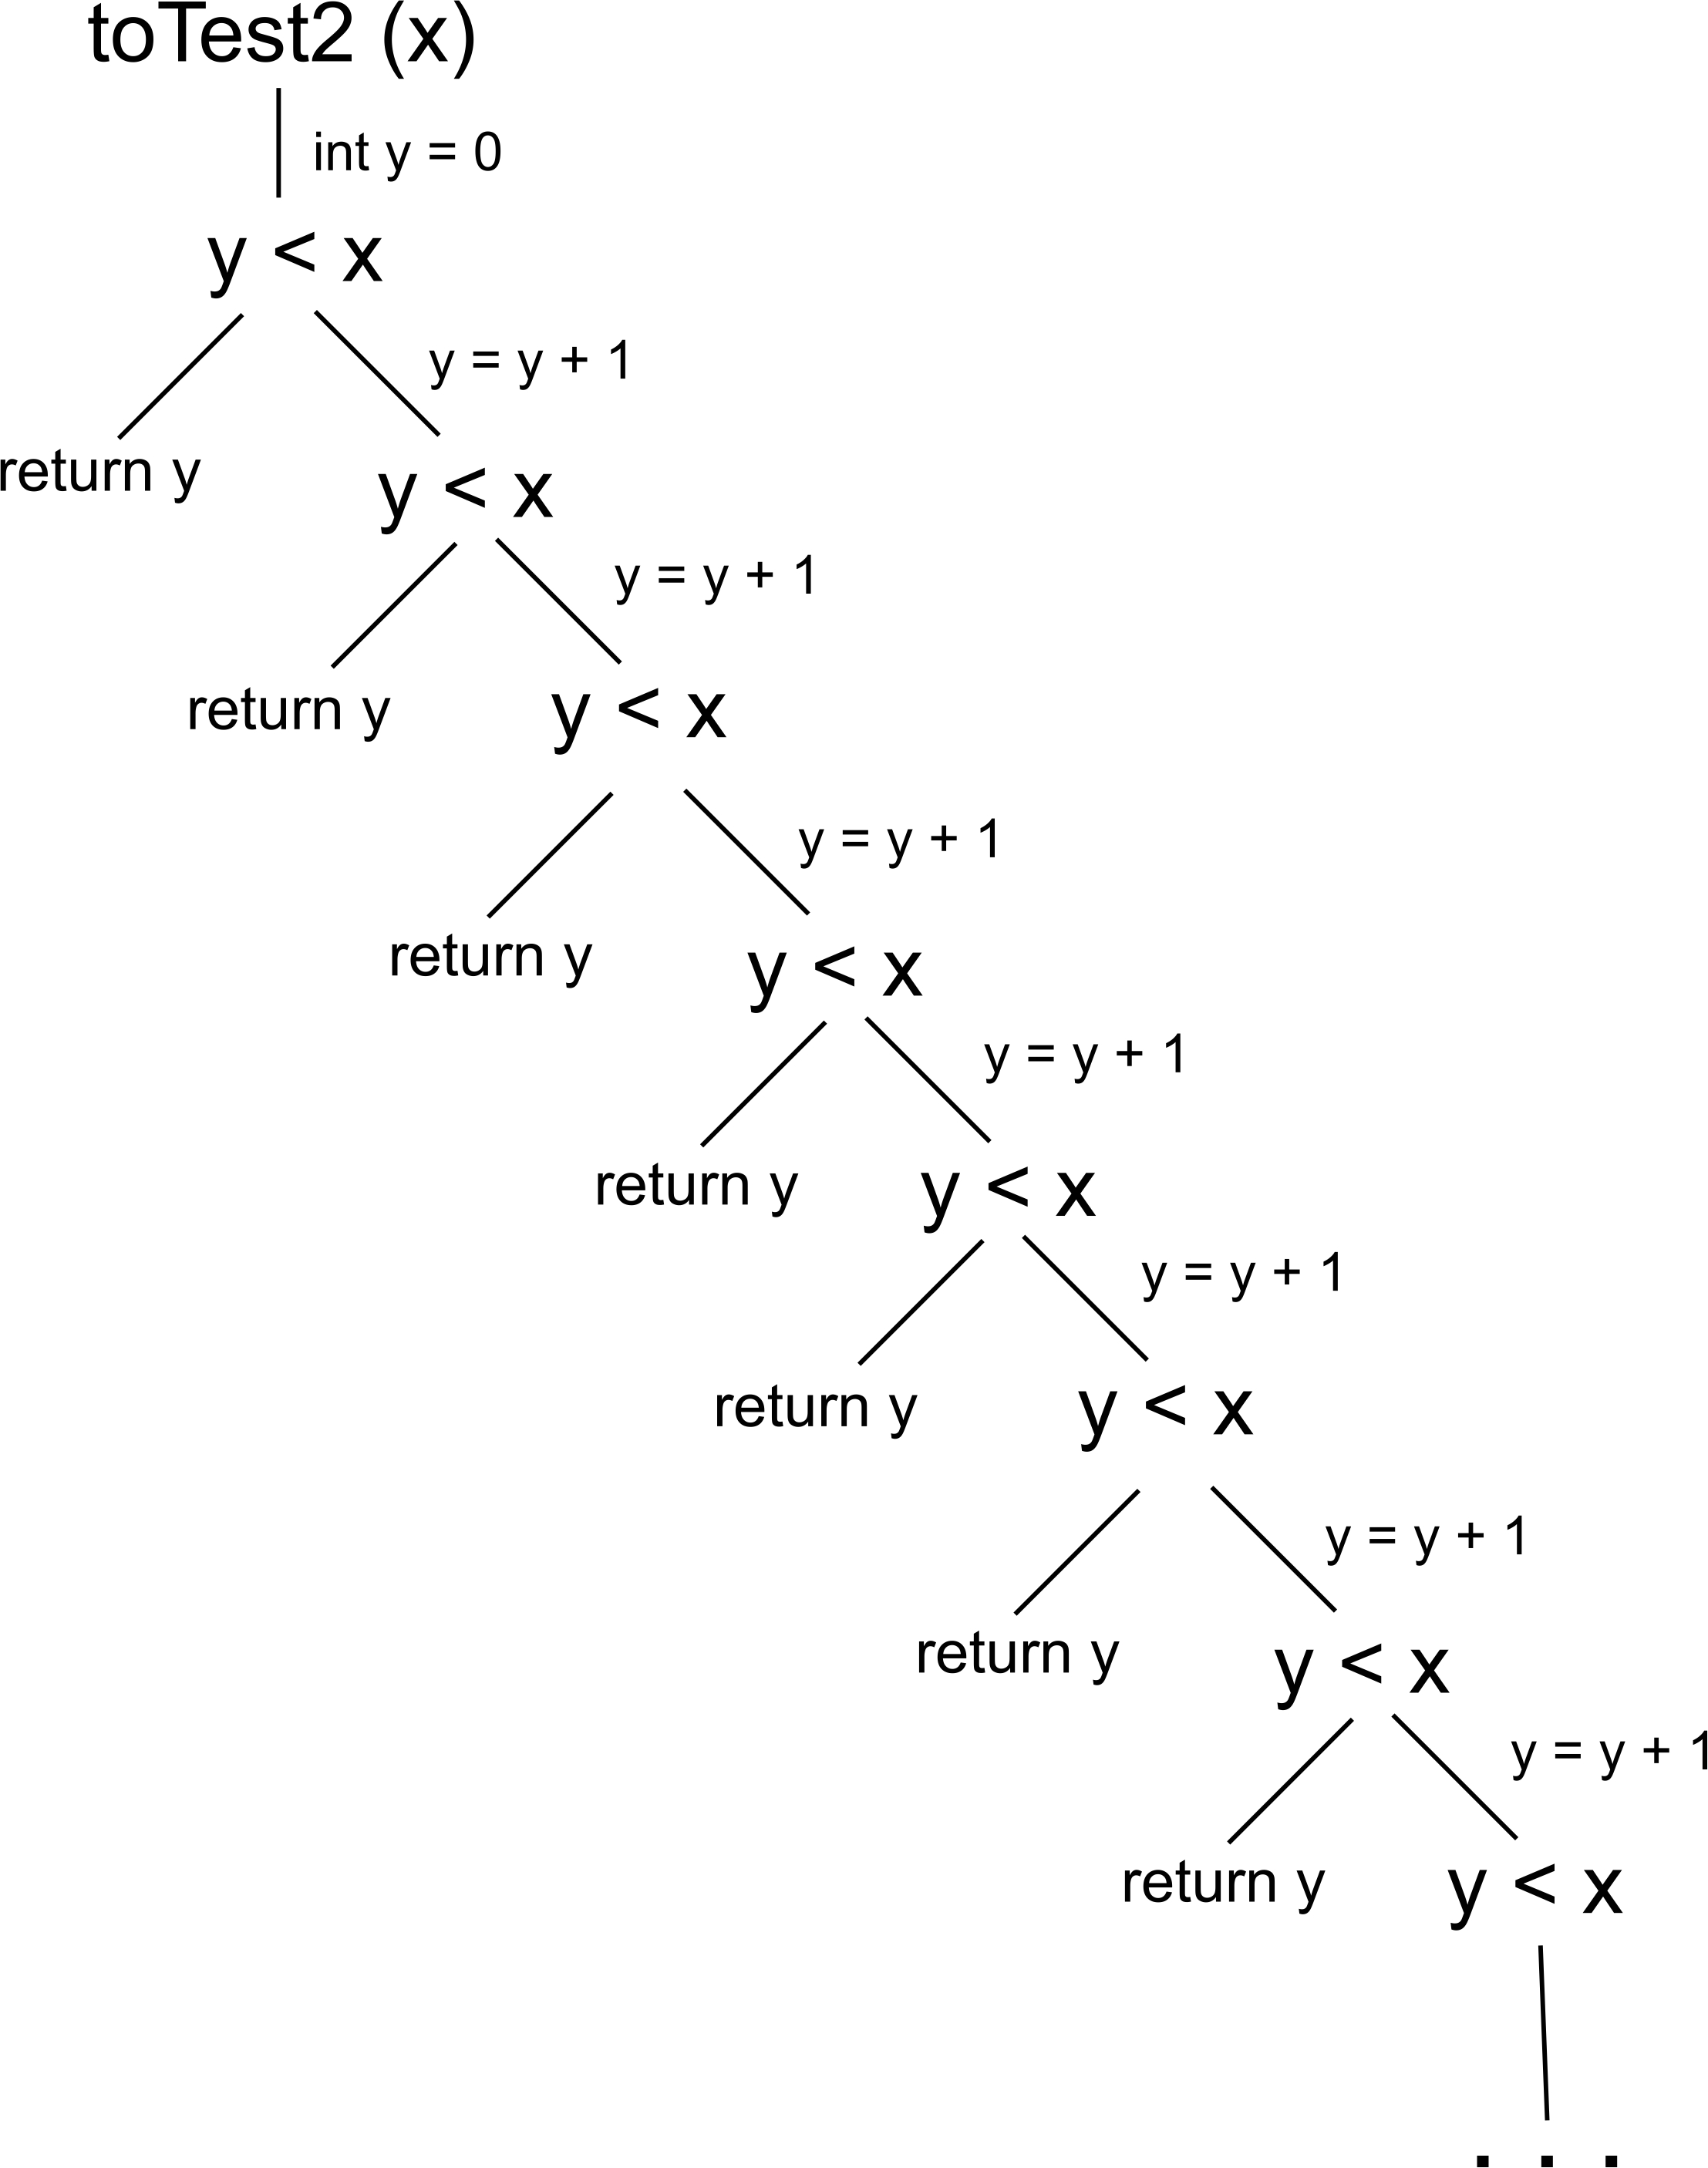
\includegraphics[width=0.95\textwidth]{cicloInf}
  \end{minipage}
  \caption{Ejemplo de ciclo infinito en la ejecución simbólica}
  \label{cicloInf}
\end{figure*}

La herramienta comienza la ejecución con $x=0$, siendo $x_0$ su variable simbólica. El while no se cumple por lo que $y=0$ y se recolecta la restricción simbólica $0 \geq x_0$.
Se niega esta condición ($0<x_0$) y se la entrega al SMT solver. Este devuelve como solución $x=1$. Nuevamente se ejecuta la función con este nuevo valor, cumpliéndose la primera vez
el while, pero no la segunda. Por lo tanto se recolectan las condiciones $0 < x_0, 1 \geq x_0$. Luego se entrega estas restricciones nuevamente al solver, negando la última
($0<x_0, 1<x_0$). Como resultado devuelve $x=2$. Se vuelve a ejecutar la función con este valor, entrando dos veces al while, por lo que el valor de $y=2$. Las restricciones simbólicas
en esta ejecución son $0<x_0, 1<x_0, 2 \geq x_0$. Se niega la última condición y el solver devuelve $x=3$. Esto permite que al ejecutar nuevamente la función con este valor se ingrese
tres veces al while, obteniendo $y=3$ y por lo tanto $0<x_0, 1<x_0, 2<x_0, 3 \geq x_0$ como restricciones simbólicas. Como es de esperar, al negar la última condición
($0<x_0, 1<x_0, 2<x_0, 3<x_0$) el solver devuelve $x=4$. Se puede observar que se ha incidido en un ciclo infinito. Por este motivo, es necesario buscar una alternativa al tratar
con ciclos.

El enfoque adoptado en este trabajo es ejecutar los ciclos a lo sumo una cantidad fija de veces k (parametrizable en la herramienta). Para esto es necesario un pre procesamiento
cuyo objetivo es reemplazar los ciclos presentes en los métodos por su equivalente en If’s anidados una cantidad fija de veces. Veámoslo mejor con un ejemplo:\\
\newline

Para \(k = 1\)
\begin{table}
\centering
\begin{tabular}{|c | c|}
\hline
\begin{lstlisting}[language=Java]
while (x < y + 1){
  x++;
}
\end{lstlisting} & 
\begin{lstlisting}[language=Java]
if (x < y + 1){
  x++;
}
\end{lstlisting}\\
\hline
\end{tabular}
\end{table}

Para \(k = 2\)
\begin{table}
\centering
\begin{tabular}{|c | c|}
\hline
\begin{lstlisting}[language=Java]
while (x < y + 1){
  x++;
}
\end{lstlisting} & 
\begin{lstlisting}[language=Java]
if (x < y + 1){
  x++;
  if (x < y +1){
    x++;
  }
}
\end{lstlisting}\\
\hline
\end{tabular}
\end{table}

Para \(k = n\)
\begin{table}
\centering
\begin{tabular}{|c | c|}
\hline
\begin{lstlisting}[language=Java]
while (x < y + 1){
  x++;
}
\end{lstlisting} & 
\begin{lstlisting}[language=Java]
if (x < y + 1){
  x++;
  //
  // (n-2 IF's)
  //
  if (x < y + 1){
    x++;
  }
}
\end{lstlisting}\\
\hline
\end{tabular}
\end{table}

De esta forma, el pre procesamiento permite modificar el programa original para evitar iteraciones infinitas.
Este programa modificado sin ciclos será sobre el cual se lleva a cabo el proceso de instrumentación que se explicará más adelante.


%%%%%%%%%%%%%%%%%%%%%%%%%%%%%%%%%%%%%%%%%%%%%%%%%%%%%%%%%%%%%%%%%%%%%%%%
%				Descripción del método		       %
%%%%%%%%%%%%%%%%%%%%%%%%%%%%%%%%%%%%%%%%%%%%%%%%%%%%%%%%%%%%%%%%%%%%%%%%
\section{Descripción del método}
El objetivo del prototipo de la herramienta desarrollada es generar casos de test para una función/método escrito en lenguaje Java que tenga parámetros de tipo
entero. En otras palabras, la herramienta recibe como input un programa y devuelve una clase java con casos de test para dicha función, lista para ejecutar con JUnit.

Para lograrlo se empleó la técnica conocida como ejecución concólica, donde se conjuga la ejecución de un programa, cuyos inputs son valores concretos,
con la representación simbólica de estos, y se registran las condiciones del programa (restricciones) utilizando los valores simbólicos de los parámetros.
Esto se logra para cada camino posible dentro del árbol de ejecución del programa. Luego de una ejecución para valores concretos, se tiene un conjunto de
ecuaciones, de las cuales se niega la última de ellas además de marcarla como ya utilizada. Luego, este nuevo conjunto de ecuaciones representará un camino
diferente en el árbol de ejecución. Para obtener valores concretos que permitan al programa ir por dicho camino, el conjunto de ecuaciones son analizadas
con un SMT solver, Z3 \cite{z3solver}, cuyo output serán los valores concretos deseados (una clase de valores que representen dichas restricciones). Con estos valores se
vuelve a ejecutar el programa, obteniendo un nuevo conjunto de ecuaciones o restricciones simbólicas que representa un camino diferente del árbol de ejecución.
Este proceso finaliza luego de obtener valores concretos para cada camino diferente. Una vez que se obtienen los valores concretos que permiten ejecutar todo el
árbol de ejecución, se genera un test por cada conjunto de valores.

Para obtener el conjunto de restricciones con la representación simbólica de los parámetros de entrada de la función, es necesario instrumentar el programa.
Spoon \cite{spoon}, una herramienta para analizar y transformar código fuente Java, es la herramienta utilizada para la instrumentación.
Este es un proceso complejo que se detallará en las subsecciones siguientes.
En la figura \ref{fig:procesosRealizados} se puede observar un esquema general de los procesos que se realizan.

\begin{figure}
\centering
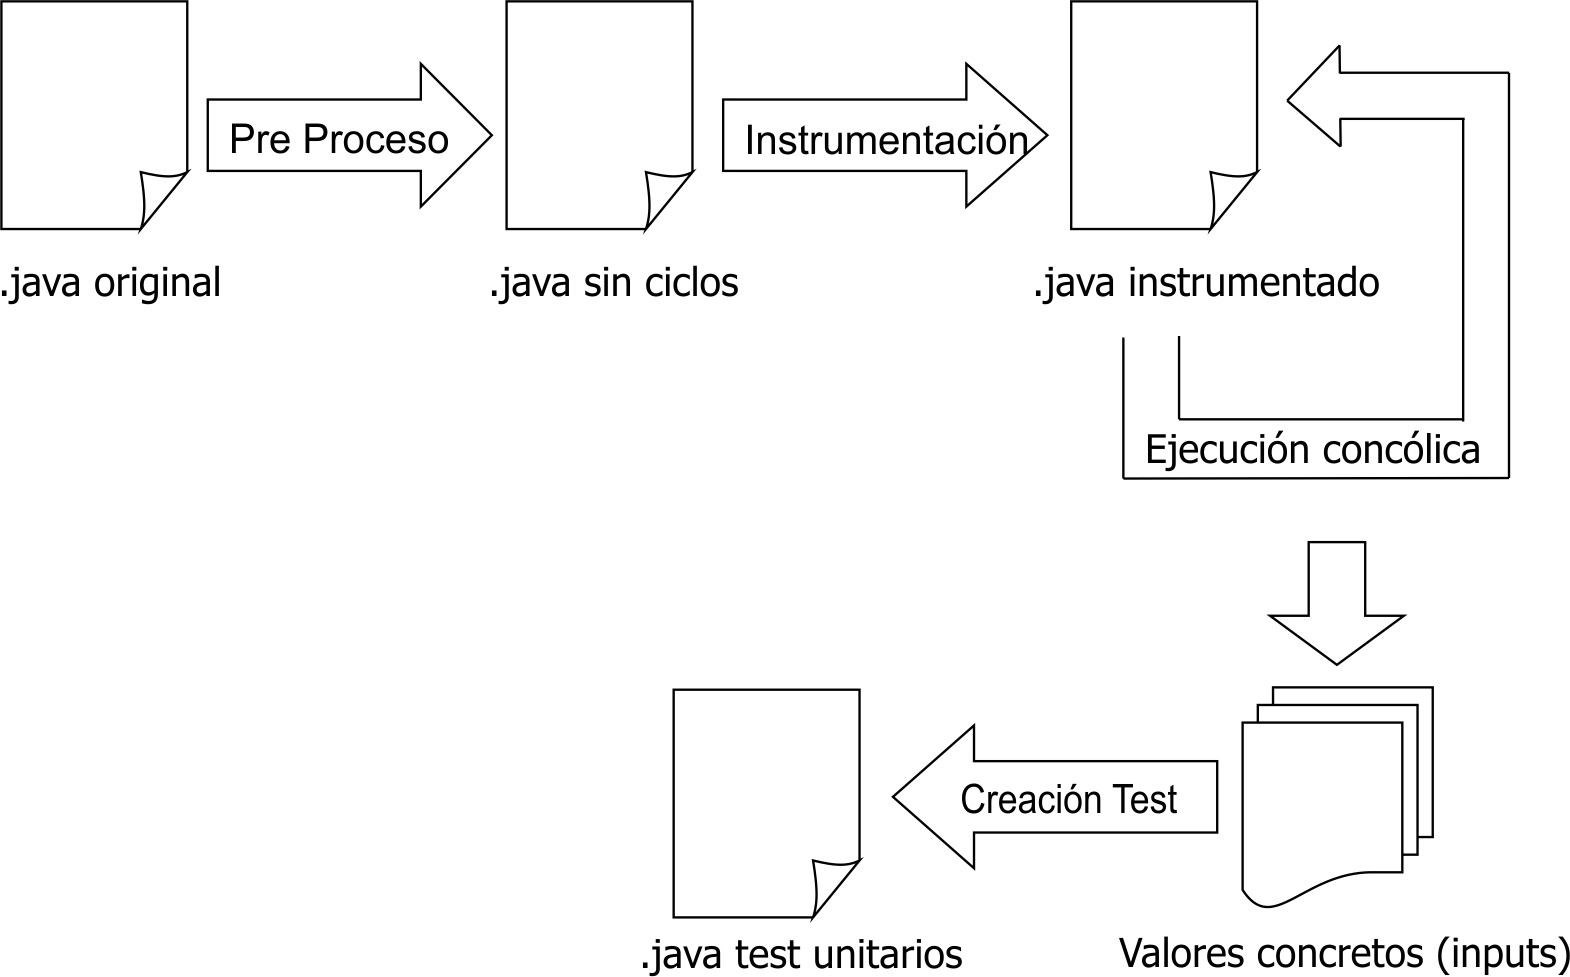
\includegraphics[width=0.85\textwidth]{procesosRealizados}
\caption{Esquema de los procesos realizados para generar los casos de test}
\label{fig:procesosRealizados}
\end{figure}

%%%%%%%%%%%%%%%%%%%%%%%%%%%%%%%%%%%%%%%%%%%%%%%%%%%%%%%%%%%%%%%%%%%%%%%%
%				Instrumentación 		       %
%%%%%%%%%%%%%%%%%%%%%%%%%%%%%%%%%%%%%%%%%%%%%%%%%%%%%%%%%%%%%%%%%%%%%%%%
\subsection{Instrumentación}
Como se mencionó antes, el objetivo de la instrumentación es obtener todas las restricciones simbólicas de los diferentes caminos del árbol de
ejecución para conseguir valores concretos que ejecuten todos los caminos posibles. Esto se logra modificando el programa sin cambiar su semántica original
pero agregando sentencias. Estas permiten recolectar restricciones simbólicas en base a los parámetros simbólicos de la función teniendo en cuenta las asignaciones
y las estructuras tipo condicionales e iterativas. Una vez finalizada la instrumentación, el programa a ejecutar es el instrumentado.
El proceso de instrumentación se realiza tomando como input el programa modificado con el pre proceso explicado en el apartado número \ref{sec:loopProblem}
debido al problema con los ciclos. De esta forma, el programa a instrumentar en lugar de contener ciclos, contiene una cantidad fija de If’s en su lugar.
La instrumentación afecta tanto a la clase como a los métodos a testear. A continuación se presenta un resumen de los procesos que lleva a cabo la instrumentación:

\begin{itemize}
  \item \underline{Asignaciones}: se detectan y registran todas las asignaciones en el método, incluyendo declaraciones locales con algún valor asignado. Luego
  de cada asignación, se agregan las sentencias necesarias para actualizar en el mapa descrito anteriormente los valores simbólicos de las variables.
  Por ejemplo, para $x=2, y=10$ el Mapa $\delta$ se comporta de la forma que ilusta el siguiente cuadro. Nótese que la segunda columna representa el momento
  inmediatamente posterior a la ejecución del código de la primer columna asociada.
      \begin{table}
	\centering
	\begin{tabular}{|m{5.5cm} | m{5cm}|}
	  \hline
	  \texttt{public Integer m(int x, int y) \{}  & $\delta$ = \{$x \mapsto x_0$; $y \mapsto y_0$\}\\
	  \hline
	  \ \ \texttt{x = x +3;} 		      & $\delta$ = \{$x \mapsto x_0 + 3$; $y \mapsto y_0$\}\\
	  \hline
	  \ \ \texttt{if (x $\geq$ y ) \{}	      &  \\
	  \hline
	  \ \ \ \ \texttt{x = x +78;} 		      & \\
	  \hline
	  \ \ \ \ \texttt{return x;} 		      & \\
	  \hline
	  \ \ \texttt{\}} 			      & \\
	  \hline
	  \ \ \texttt{y = x - 2;} 		      & $\delta$ = \{$x \mapsto x_0 + 3$; $y \mapsto x_0 +3 - 2$\}\\
	  \hline
	  \ \ \texttt{return y}; 		      & \\
	  \hline
	  \texttt{\}} 				      & \\
	  \hline
	\end{tabular}
	\centering
	\caption{Asignaciones con su representación simbólica dado por el Mapa $\delta$. Método ejecutado con ($x=2, y=10$)}
      \end{table}
      
  \item \underline{Sentencias IF’s}: el árbol de ejecución está representado por los diferentes caminos posibles que puede tener un programa. Estos están determinados por las
  estructuras condicionales presentes en el código. Un método sin condicionales, es un método con un único camino posible a ejecutar. Por esta razón, las restricciones simbólicas
  mencionadas están determinadas por las sentencias condicionales cuyos valores son los valores simbólicos de los parámetros de entrada, cuando corresponda. En la figura
  \ref{arbolEjecucion} se puede observar un ejemplo de un método con su correspondiente árbol de ejecución.
  
  A continuación se presenta un ejemplo de cómo se recolectan las restricciones simbólicas que luego serán enviadas a un solver para obtener valores concretos.
  Cabe destacar que las restricciones simbólicas se recolectan para una ejecución concreta del método a testear, es decir, con valores concretos para cada parámetro de la función.
  
      \begin{table}
	\centering
	\begin{tabular}{|m{5.5cm} | m{6cm}|}
	  \hline
	  \texttt{public Integer m1(int $x$, int $y$)} \{  & \ \ $\delta$ = \{$x \mapsto x_0$; $y \mapsto y_0$\}\\
	  \hline
	  \ \ \texttt{x = x * 3;}                          & \ \ $\delta$ = \{$x \mapsto x_0*3$; $y \mapsto y_0$\}\\
	  \hline
	  \ \ \texttt{if (x == y)) \{} 	                   & \ \ $\alpha$ = ($x_0*3 == y_0$)\\
	  \hline
	  \ \ \ \ \texttt{x = x+y;} 		           & \ \ $\delta$ = \{$x \mapsto x_0*3+y$; $y \mapsto y_0$\}\\
	  \hline
	  \ \ \ \ \texttt{if (x $\geq$ 100\ \&\&\ y > 0)}  & \ $\alpha$ = ($x_0*3 == y_0$, !($x_0*3+y_0 \geq 100\ \&\&\ y_0>0$))\\
	  \hline
	  \ \ \ \ \texttt{return x;} 			   & \\
	  \hline
	  \ \ \} 				  	   & \\
	  \hline
	  \ \ \texttt{if (x \% 2 == 0)}			   & \ $\alpha$ = ($x_0*3 == y_0$, !($x_0*3+y_0 \geq 100\ \&\&\ y_0>0$, ($x_0*3+y_0$)$\%2$))\\
	  \hline
	  \ \ \ \ \texttt{return x}; 			   & \\
	  \hline
	  \ \ \texttt{return y}; 		 	   & \\
	  \hline
	  \} 						   & \\
	  \hline
	\end{tabular}
	\caption{Ejemplo de recolección de restricciones simbólicas $\alpha$. El Mapa lógico $\delta$ actualiza los valores simbólicos de los
	parámetros de entrada de la función. Método ejecutado con ($x=0, y=0$)}
      \end{table}
      Los restricciones $\alpha$ serán las enviadas al SMT Solver para obtener valores concretos para $x$ e $y$.
      
\end{itemize}


%%%%%%%%%%%%%%%%%%%%%%%%%%%%%%%%%%%%%%%%%%%%%%%%%%%%%%%%%%%%%%%%%%%%%%%%
%				SMT solver	        	       %
%%%%%%%%%%%%%%%%%%%%%%%%%%%%%%%%%%%%%%%%%%%%%%%%%%%%%%%%%%%%%%%%%%%%%%%%
\subsection{SMT Solver}
El SMT solver utilizado en este trabajo es el Z3, desarrollado por Microsoft Research. El uso de este componente es fundamental en el desarrollo de la ejecución concólica para
obtener los valores a utilizar en los casos de test generados. Este solver permite chequear la satisfacibilidad de fórmulas lógicas sobre una o más teorías, otorgando valores que
satisfagan dichas fórmulas cuando sea posible.

El uso de Z3 en el desarrollo de la herramienta se ha mencionado a lo largo del presente artículo: las restricciones simbólicas recolectadas mediante la ejecución del código
instrumentado -un método particular con parámetros enteros- se envían a Z3 luego de negar la última de estas restricciones. Este solver las procesa y, de ser posible, devuelve
valores concretos que satisfagan dichas restricciones (valores concretos para las variables simbólicas). Estos valores son utilizados como input del método instrumentado para
recorrer un camino alternativo al anterior, recogiendo nuevas restricciones simbólicas que serán procesadas por Z3 (siempre negando la última restricción), hasta que se hayan
procesado todas estas restricciones.

Usar un SMT solver tiene como principal ventaja que permite obtener valores concretos que aseguren recorrer todas las ramas alcanzables del árbol de ejecución, obteniendo 100\%
de cobertura en los test -siempre y cuando no exista código muerto en el programa-. Sin embargo, presenta algunas desventajas en cuanto a limitaciones que se detallan en el
apartado siguiente.

%%%%%%%%%%%%%%%%%%%%%%%%%%%%%%%%%%%%%%%%%%%%%%%%%%%%%%%%%%%%%%%%%%%%%%%%
%				Limitaciones       		       %
%%%%%%%%%%%%%%%%%%%%%%%%%%%%%%%%%%%%%%%%%%%%%%%%%%%%%%%%%%%%%%%%%%%%%%%%
\section{Limitaciones}
A continuación se describe brevemente limitaciones que abordan dos cuestiones: limitaciones inherentes a la ejecución concólica y limitaciones del prototipo de la herramienta
desarrollado que pueden superarse.

Uno de los principales límites de la ejecución concólica es la dependencia de un SMT Solver que permita resolver las restricciones simbólicas. Existe una restricción sobre las
teorías que pueden incluirse que depende del SMT solver subyacente. Si bien se ha avanzado en las teorías que manejan (enteros, reales, strings, arrays, etc.), aún existen tipos
no soportados. Otra limitación es el tiempo que puede demandar el solver en encontrar una solución para ciertas ecuaciones, como por ejemplo ciertas restricciones lineales enteras
con complejidad exponencial.

Por otro lado, existen limitaciones del prototipo desarrollado que pueden resolverse. Por ejemplo, esta herramienta actualmente sólo puede generar casos de test para métodos cuyos
parámetros y restricciones en el código son de tipo entero. Además soporta sólo las operaciones suma (+), resta (-), división (/), producto (*) y módulo (\%).

%%%%%%%%%%%%%%%%%%%%%%%%%%%%%%%%%%%%%%%%%%%%%%%%%%%%%%%%%%%%%%%%%%%%%%%%
%				Conclusiones y continuación	       %
%%%%%%%%%%%%%%%%%%%%%%%%%%%%%%%%%%%%%%%%%%%%%%%%%%%%%%%%%%%%%%%%%%%%%%%%
\section{Conclusiones y continuación}


%%%%%%%%%%%%%%%%%%%%%%%%%%%%%%%%%%%%%%%%%%%%%%%%%%%%%%%%%%%%%%%%%%%%%%%%
%				Referencias 			       %
%%%%%%%%%%%%%%%%%%%%%%%%%%%%%%%%%%%%%%%%%%%%%%%%%%%%%%%%%%%%%%%%%%%%%%%%

\begin{thebibliography}{X}
\bibitem{dart} \textsc{P. Godefroid}, \textsc{N. Klarlund} y \textsc{K. Sen}. \textit{DART: Directed automated random testing}. 2005.
\bibitem{cute} \textsc{K. Sen}, \textsc{D. Marinov} y \textsc{G. Agha}. \textit{CUTE: A concolic unit testing engine for C}. 2005.
\bibitem{symb} \textsc{King, James C}. \textit{Symbolic Execution and Program Testing}. 1976.
\bibitem{spoon} \textsc{Renaud Pawlak}, \textsc{Carlos Noguera} y \textsc{Nicolas Petitprez}. \textit{Spoon: Program Analysis and Transformation in Java}, [Research Report] RR-5901, Inria. 2006.
\bibitem{z3solver} \textsc{Leonardo de Moura} y \textsc{Nikolaj Bjørner}. \textit{Z3: An Efficient SMT Solver}, Microsoft Research. 2008.
\bibitem{revSimb} \textsc{Cristian L. Vidal}, \textsc{Rodolfo F. Schmal}, \textsc{Sabino Rivero} y \textsc{Rodolfo H. Villarroel}. \textit{Una Revisión sobre la Ejecución Simbólica de Programas Computacionales}. 2014
\bibitem{econImpact} \textsc{Gregory Tassey}. \textit{The Economic Impacts of Inadequate Infrastructure for Software Testing}. 2002.
\bibitem{sym2con} \textsc{Daniel Paqué}. \textit{From Symbolic Execution to  Concolic Testing}. 2014.
\bibitem{jcute} \textsc{K. Sen} y \textsc{G. Agha}. \textit{CUTE and jCUTE: Concolic Unit Testing and Explicit Path Model-Checking Tools}. 2005.
\end{thebibliography}



\end{document}
